%!TEX program = xelatex
\documentclass[a5paper,12pt,onecolumn]{article}

\usepackage{fontspec}
\setmainfont{Alegreya}
\setmonofont{Inconsolata}
\setsansfont{Averia Sans}

\usepackage[
	papersize={396bp, 596bp},
	ignoreheadfoot,
	total={324bp, 524bp},
	% showframe,
	left = 36bp,
	top = 36bp,
	twoside,
	marginpar = 1in,
	footskip = 2\baselineskip,
]{geometry}

% setup headings
\usepackage{fancyhdr}
\fancypagestyle{plain}{%
	\fancyhf{}
	\fancyfoot[C]{\sf–~\thepage~–}
	\renewcommand\headrulewidth{0pt}
	\renewcommand\footrulewidth{0pt}
}
\pagestyle{plain}

\usepackage{graphicx}
\setkeys{Gin}{width=\linewidth,height=0.915\textheight,keepaspectratio}

\usepackage[final]{listings}
\lstset{
	basicstyle=\footnotesize,
	numbers=left,
	breaklines=true,
	frame=leftline,
	captionpos=b,
	tabsize=2,
	breakatwhitespace=true,
}
\def\code#1{\mbox{\lstinline{#1}}}

\lstnewenvironment{cli}{\lstset{numbers=none, frame=off,}}{}

\usepackage{amsmath}
\usepackage{amsfonts}
\newtheorem{definition}{Definition}

\usepackage{cite}
\usepackage{hyperref}
\usepackage{url}
\usepackage{microtype}
\usepackage{float}

% set the headings
\makeatletter
\renewcommand\section{\@startsection {section}{1}{\z@}%
	{-6.5ex \@plus -1ex \@minus -.2ex}%
	{3.0ex}%
	{\sf\Large}}
\renewcommand\subsection{\@startsection {subsection}{2}{\z@}%
	{-3.5ex \@plus -1ex \@minus -.2ex}%
	{1.5ex}%
	{\sf\large}}
\renewcommand\subsubsection{\@startsection{subsubsection}{3}{\z@}%
	{-5.25ex\@plus -1ex \@minus -.2ex}%
	{1.0ex}%
	{\sf}}
\makeatother

\begin{document}

\begin{center}
	\sf\Huge Seed Tutorial
\end{center}

This tutorial will introduce you to Seed and its prototype. You will learn how to build services, use the service monitor, apply transformations, write a browser-based client, and write map and reduce functions. The working example for this tutorial is a key-value store (kvs).

\section{Prerequisites}

Several things are needed before we can get started.

\begin{itemize}
\item Go \url{http://golang.org}
\item Gnuplot
\item Seed \url{https://github.com/nathankerr/seed}
\item A web browser (tested in Safari, Chrome, and Firefox)
\item Some knowledge of command lines, go, javascript, html, websockets, json, and services.
\end{itemize}

Seed will work on Windows, OS X, and Linux. The command line instructions are geared toward OS X and Linux. If you are using Windows, please use \code{cmd} or write \code{\%--} before command line arguments (if using PowerShell). Also, change \code{/} to \code{\\}.

\section{Getting Started}

Start by making a new directory to work in:

\begin{cli}
mkdir seed-tutorial; cd seed-tutorial
\end{cli}

Create a file, \code{kvs.seed}, with the following contents (don't include the line numbers).

\lstinputlisting{start/kvs.seed}

This file defines the core of a key-value store service. Line~1 describes a table called \code{kvstate} with a single key column called \code{key} and a single value column called \code{value}.

\section{Starting the Service}

Start the service by running:

\begin{cli}
seed -sleep 0.5s -monitor :8000 -execute kvs.seed
\end{cli}

\code{-sleep 0.5s} will sleep half a second in between time steps. This slows things down enough so that we can see what is happening in the service instance. A sleep value is needed when using the monitor to limit the data the web browser must process.

\code{-monitor :8000} starts the debugging monitor on port 8000. To restrict access to localhost, use \code{-monitor localhost:8000}.

\code{-execute} starts the service using the built in interpreter.

\section{The Monitor}

The Seed prototype includes a monitor that allows you to see what is happening in your service. Now that the service has been started, the monitor can be accessed at \url{http://localhost:8000} using your favorite web browser:

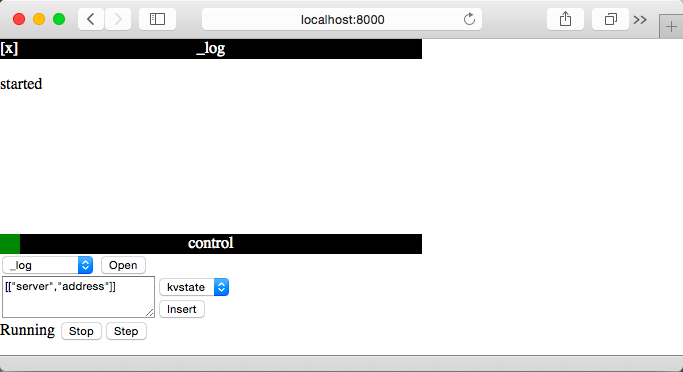
\includegraphics{start/monitor.png}

The debug monitor presents a view of the state of the service instance. The control area has controls for controlling the monitor.

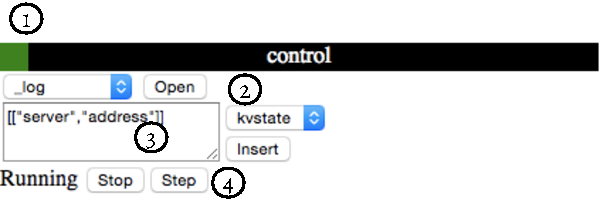
\includegraphics{start/control}

\begin{enumerate}
\item Green shows the monitor is connected; red disconnected.
\item Access to available views. Select the desired view and press open.
\item Control to insert data into a collection. Data is encoded in JSON as an array of arrays. \code{"server"} and \code{"address"} are special values that are translated into the server and client addresses respectfully.
\item Execution control. Start and stop the service, and step through the parts of the time step.
\end{enumerate}

The rest of the monitor area is for the views. Click on the name of the view to put it in the main area (on the left, where \code{_log} is); \code{[x]} to close the view. Views beginning with underscores are special.

\begin{description}
\item[\_log] The monitor log
\item[\_service] The service that is running (expressed in Seed)
\item[\_graph] The flow graph of the running service. Rule numbers in the graph correspond to those in \code{_service}.
\item[\_time] The time spent on the last timestep
\end{description}

Views not beginning with underscores correspond to collections (e.g., tables, inputs, outputs) in the service.

You can use the monitor to insert data into \code{kvstate}. The displayed order of rows for \code{kvstate} might fluctuate. This is due to the unordered nature of collections\footnote{Collections are implemented using Go's map datatype. When Go maps contain a small number of keys, the order is randomized when accessing all the keys so that developers will not accidentally depend on the implementation's natural ordering of this unordered dataset.}.

You can stop the service at any time by pressing ctrl-C in the command line.

\section{KVS Put Operation}

We will now expand the core of our kvs service by adding a put operation. Put inserts key-value pairs into kvstate.

Update \code{kvs.seed} to match:

\lstinputlisting{put/kvs.seed}

Line~3 defines an input called \code{kvput} that contains two columns: \code{key} and \code{value}. Like all collections, inputs have key and data columns. Input and output collections define the flow of data into and out of a service. These collection types are not network accessible.

Line~4 is a rule which projects the columns in \code{kvput} and then upserts (\code{<+-}) the resulting set into \code{kvstate}.

Start the service with:

\begin{cli}
seed -sleep 0.5s -monitor :8000 -execute kvs.seed
\end{cli}

Insert stuff into kvput and watch how it flows to kvstate. Try using various values to see how things work. Also look at the \code{_service} and \code{_graph} views to see how they relate. Note that no transformations have been applied (we will transform the service in later steps).

\section{Put Client}

We will now build a client for the service. First the service needs a network interface. When starting the service, the network interface is added by using the \code{network} transformation:

\begin{cli}
seed -sleep 0.5s -monitor :8000 -execute -transformations network kvs.seed
\end{cli}

Check the service's \code{_service} and \code{_graph} views to see the results of the transformation.

The client will use a custom json over webservices protocol. This protocol was implemented to allow web browser based clients.

The client is implemented as a static web page (\code{index.html}):

\lstinputlisting{client/index.html}

The client is initialized with the init function on Lines~26-48 this is ran on load (Line~50). A websocket connection is setup in Lines~32-35. A pseudorandom address is then created and sent to the server. This address will be used as the client address for Channel based communication and lasts as long as the websocket.

When initialization is completed, the connection indicator (Line~54) is turned green. When the websocket is closed, the connection will turn red (Line~35, Lines~10-12).

When the put button in the form is pressed (or the form is otherwise submitted), the send function in Lines~14-24 is executed. This function simply builds, serializes, and sends the data over the websocket to the server.

Because web browsers don't like allowing websocket access from pages loaded from the local file system, we need a simple web server:

\lstinputlisting{client/server.go}

Start the client web server by:

\begin{cli}
go run server.go
\end{cli}

And then open your browser to \url{http://localhost:4000}. As usual, the server will bind to all your computer's network interfaces. To restrict it, change \code{addr} on Line~8 to \code{localhost:4000}.

To see a more advanced client that also handles results, look at the example time service client's implementation \footnote{\url{services/time} in the seed repository}.

\section{Replication}

We will now setup and run a replicated kvs. No changes to any code are needed to do this.

Start the first replica:

\begin{cli}
seed -sleep 0.5s -monitor :8000 -execute -transformations "network replicate" -address :3000 kvs.seed
\end{cli}

Insert \code{[["127.0.0.1:3001"]]} into \code{:8000}'s \code{kvstate_replicants} using the monitor.

Also, set up the views as follows:

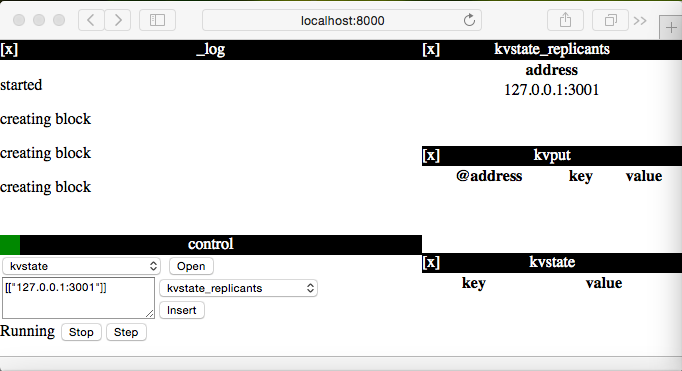
\includegraphics{replicate/first.png}

Start the second replica:

\begin{cli}
seed -sleep 0.5s -monitor :8001 -execute -transformations "network replicate" -address :3001 kvs.seed
\end{cli}

Insert \code{[["127.0.0.1:3000"]]} into \code{:8001}'s \code{kvstate_replicants} using the monitor.

Also, set up the views as follows:

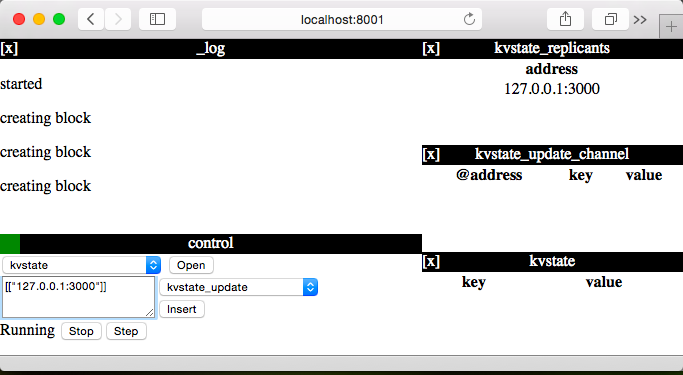
\includegraphics{replicate/second.png}

Start the client (will connect to \code{:3000}):

\begin{cli}
go run server.go
\end{cli}

If you have the two replica monitors and the client in different windows, you can watch the entire progression.

Put some value into the client and watch as it first hits the first replica and then the second.

Note that due to the transformations, no changes were needed to \code{kvs.seed} or the client to enable replication. However, while the client will only connect to one of the replicas, this could be resolved by using a load balancer.

\section{Compiling Services}

Up to this point the services have been interpreted by the \code{seed} tool. Now we will compile the service. This is done in two steps:

\begin{enumerate}
\item Use the \code{seed} tool to perform desired transformations and output \code{go} source code for the service.
\item Use \code{go} to compile the resulting code.
\end{enumerate}

This process will be done for the replicated kvs. First,

\begin{cli}
seed -transformations "network replicate" -t go kvs.seed
\end{cli}

applies the network and replicate transformations a before. However, all execution options have been removed and replaced with \code{-t go}, which tells \code{seed} to output \code{go} source code. By default this is done is a directory called \code{build}. To compile your replicated kvs:

\begin{cli}
cd build
go build -o kvs
\end{cli}

This first moves to the build directory and then uses \code{go build} to build all the \code{go} files in that directory and name the resulting executable \code{kvs} (the default is the name of the directory).

The service can then be started with:

\begin{cli}
./kvs -sleep 0.5s -monitor :8000 -address :3000
\end{cli}

The same execution options (e.g., sleep, monitor, address) can be used as before.

\section{Using Map Functions}

To learn how to use map functions in Seed, we will extend the kvs service. The map function we will build converts a string to upper-case characters.

Map functions are not implemented in Seed, but in the host language (in this case, \code{go}). As the function is implemented in the host language, it can do any things the host language can.

First modify \code{kvs.seed} to:

\lstinputlisting{map/kvs.seed}

Line~6 defines a new table where we will keep the key, uppercased-value pairs. Line~7 take values from \code{kvput} like we did on Line~4, but instead of using the raw \code{kvput.value}, it runs a map function \code{upper} with a single argument \code{kvput.value}. Map functions and their arguments are surrounded by \code{( )}. Arguments are space delimited.

Define the map function in \code{upper.go}:

\lstinputlisting{map/upper.go}

Line~1 declares the contents of the file to be part of the main package. Lines~3-7 import the two packages we will use to define the map function. We will use \code{strings.ToUpper} to uppercase \code{kvput.value}. The seed package is used to access the types needed by a map function. A map function is defined as \code{func(Tuple) Element}. A \code{Tuple} is \code{[]interface\{\}} and will contain the arguments to the map function for that row. An \code{Element} is \code{interface\{\}} and will be used in the place of the map call.

The function itself is deceptively simple. \code{input[0]} grabs the first value in the input tuple. In this case, there should only be one value, as we only specified one argument to \code{upper}. If there were more arguments, they would appear in \code{input}.

\code{input[0].(string)} asserts that \code{input[0]} is a string. This is needed because a \code{Tuple} can contain any type. The actual type is dependent on the data sent to the server (JSON over websockets) and the type the JSON unmarshaller uses for that data. If some data that is not unmarshalled as a string, such a number, is there, the server will panic. Thus a better implementation would need to handle those cases.

Finally, \code{strings.ToUpper} converts that value to its upper case value, which is then returned. The executor uses the returned value to fill the map function's place in the result tuple before inserting it into \code{upper}.

The whole build and run process can be done as follows:

\begin{cli}
seed -t go -transformations network kvs.seed
cp upper.go build/
cd build
go build -o kvs
./kvs -sleep 0.5s -monitor :8000
\end{cli}

Use the monitor (and the client if you like) to see that the map function is called and its results.

\section{Using Reduce Functions}

We will now use a reduce function. Reduce functions are similar to map functions, except they take an array of tuples instead of a single tuple as input.

The example we will build counts the number of keys that have the same value.

First modify \code{kvs.seed}:

\lstinputlisting{reduce/kvs.seed}

Lines~6-7 define our new collection and rule. A scratch collection is used so that other operations on \code{kvstate} such a removing tuples will not cause incorrect values in our count collection.

The syntax for the reduce function \code{count} is similar to that of a map function, except that \code{\{ \}} are used instead of \code{( )}. Fields in the intension other than the reduce function group\footnote{Similar to how GROUP BY is used in combination with an aggregate function in SQL.} the rows passed to the function. In this case, all the \code{kvstate.key}s that have the same \code{kvstate.value} are passed to the \code{count} reduce function. \code{count} is called for each unique \code{kvstate.value}.

The reduce function is implemented in \code{count.go}:

\lstinputlisting{reduce/count.go}

A reduce function is a \code{func([]Tuple) Element}. Lines~5-7 implement \code{count}. In this example we don't have to worry about the data in the slice of tuples, as we just want its length (count). Line~6 returns the length of the input slice.

Building and running the service can be done as follows:

\begin{cli}
seed -t go -transformations network kvs.seed
cp count.go build/
cd build
go build -o kvs
./kvs -sleep 0.5s -monitor :8000 -address :3000
\end{cli}

Use the monitor (and the client if you like) to explore the behavior of the reduce function.

\end{document}
